\documentclass[../main.tex]{subfiles}

\begin{document}
		\section{Diskussion und Ausblick}
	
	\subsection{Sprint 0 Meeting}
	\begin{itemize}
		\item Angular Demo von  Herr Bachmann TodoAngular.
		\begin{itemize}
			\item In Github Frontend - Package.JSON ist alles vorhanden was zu diesem Thema als Wissen benötigt wird.
		\end{itemize}
		\item Hosting kann von Herrn Bachmann übernommen werden.
		\begin{itemize}
			\item Hierfür muss entweder ein Dockercontainer für das Frontend und Backend respektive erstellt werden, oder für das Frontend und Backend kombiniert.
		\end{itemize}
		\item Cloud Service für VM Möglichkeiten.
		\begin{itemize}
			\item Auf der Homepage \url{https://www.hetzner.com} gibt es zahlreiche kosteneffiziente und interessante Angebote für verschiedene Services.
		\end{itemize}
		\item Erstellen und diskutieren der Tasks für Sprint 1.
	\end{itemize}	
	
	\subsection{Sprint 1 Meeting}
	\begin{itemize}
		\item Durch verschiedene Versionierungen und unterschiedlichen Arbeitsstationen kam es zu einigen Problemen mit Gradle unter anderem auch Dependeciesfehler.
		\item Unter längerer Diskussion wurde beschlossen dass das Frontend und Backend in einem Dockercontainer kombiniert werden um das hosten und arbeiten zu vereinfachen.
		\item Eine kurze Dockerpräsentation auf einer virtuellen Ubuntumaschine über den aktuellen Stand wird vorgeführt.
		\item Angular Frontend steht noch offen und wird als Letztes angegangen.
		\item Ein weiterer Punkt wäre ein mögliches Treffen mit dem Team aus Wädischwil bezüglich Mockups. Um eine grobe Richtung für ungefähre GUI Vorstellungen zu bekommen oder ob dies komplett nach eigenem Ermessen erstellt werden soll.
	\end{itemize}	
	\subsection{Sprint 2 Meeting}
	\begin{itemize}
		\item Um weiter fortzufahren mit dem GUI wird eine Diskussion über das gewünschte Layout geführt. 
		\begin{itemize}
			\item Die Sensoren sollen tabellarisch aufgelistet werden. 
			\item Es soll möglichst einfach sein über einen Button einen Sensor hinzuzufügen.
			\item Die Details in den Tabellen sollen eine Funktion haben, über welche die Daten direkt in der Tabelle schnell geändert werden können.
			\item Die Reihenfolge der Tabellen soll gleich wie auf dem SC1000 bei der folgenden Abbildung gegliedert sein.
			Wie in der Abbildung ersichtlich werden die Tanks einzeln aufgezeigt mit ähnlichen Eigenschaften. 
			\begin{figure}[h]
				\centering
				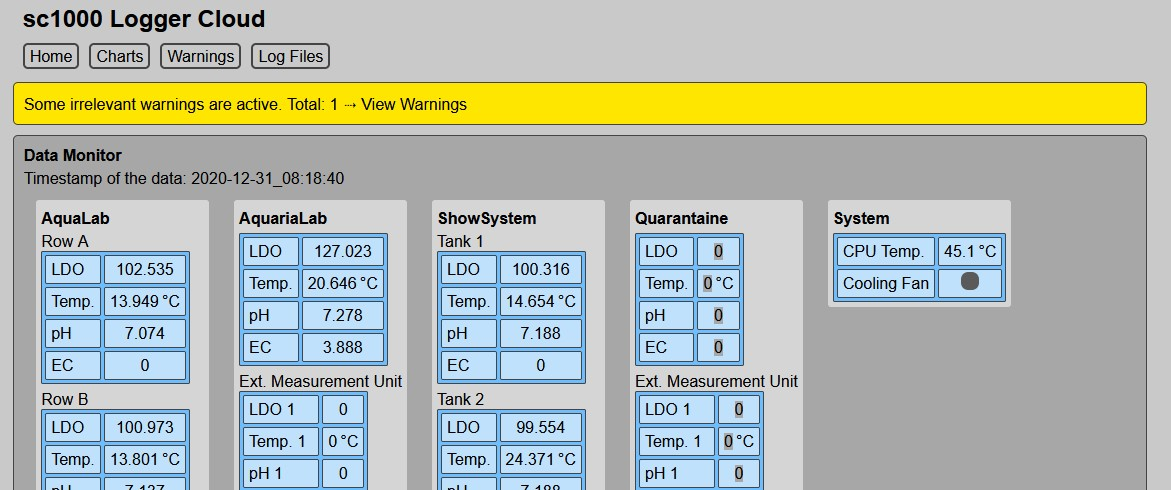
\includegraphics[scale=0.4]{SC1000_Example}
				\caption{SC1000 Screenshot}
				\label{fig:SC1000_Example}
			\end{figure}
			
			
			\item Alle Adressen der Sensoren sollen genauso im SC1000 geregelt werden können.
		\end{itemize}
		\item Der erstellte Docker Container mit dem kombinierten Frontend und Backend wird präsentiert und die Benutzung erklärt.
		\item Da die Möglichkeit besteht bei Herrn Bachmann den Docker Container vorübergehend hosten zu lassen, muss entschieden werden wie das Team aus Wädischwil danach mit dem hosten fortfahren möchten.
		\item Die Sensorendaten werden über MQTT zur Urbanblue geschickt
		\item Ein erneutes Meeting wird 2 Wochen später nochmal einberufen um die ersten Schritte des GUIs zu zeigen.
	\end{itemize}
\end{document}